\documentclass{ximera}

\graphicspath{  %% When looking for images,
{./}            %% look here first,
{./pictures/}   %% then look for a pictures folder,
{../pictures/}  %% which may be a directory up.
{../../pictures/}  %% which may be a directory up.
{../../../pictures/}  %% which may be a directory up.
{../../../../pictures/}  %% which may be a directory up.
}

\usepackage{listings}
\usepackage{circuitikz}
\usepackage{xcolor}
\usepackage{amsmath,amsthm}
\usepackage{subcaption}
\usepackage{graphicx}
\usepackage{tikz}
\usepackage{tikz-3dplot}
\usepackage{amsfonts}
\usepackage{mdframed} % For framing content
\usepackage{tikz-cd}

  \renewcommand{\vector}[1]{\left\langle #1\right\rangle}
  \newcommand{\arrowvec}[1]{{\overset{\rightharpoonup}{#1}}}
  \newcommand{\ro}{\texttt{R}}%% row operation
  \newcommand{\dotp}{\bullet}%% dot product
  \renewcommand{\l}{\ell}
  \let\defaultAnswerFormat\answerFormatBoxed
  \usetikzlibrary{calc,bending}
  \tikzset{>=stealth}
  




%make a maroon color
\definecolor{maroon}{RGB}{128,0,0}
%make a dark blue color
\definecolor{darkblue}{RGB}{0,0,139}
%define the color fourier0 to be the maroon color
\definecolor{fourier0}{RGB}{128,0,0}
%define the color fourier1 to be the dark blue color
\definecolor{fourier1}{RGB}{0,0,139}
%define the color fourier 1t to be the light blue color
\definecolor{fourier1t}{RGB}{173,216,230}
%define the color fourier2 to be the dark green color
\definecolor{fourier2}{RGB}{0,100,0}
%define teh color fourier2t to be the light green color
\definecolor{fourier2t}{RGB}{144,238,144}
%define the color fourier3 to be the dark purple color
\definecolor{fourier3}{RGB}{128,0,128}
%define the color fourier3t to be the light purple color
\definecolor{fourier3t}{RGB}{221,160,221}
%define the color fourier0t to be the red color
\definecolor{fourier0t}{RGB}{255,0,0}
%define the color fourier4 to be the orange color
\definecolor{fourier4}{RGB}{255,165,0}
%define the color fourier4t to be the darker orange color
\definecolor{fourier4t}{RGB}{255,215,0}
%define the color fourier5 to be the yellow color
\definecolor{fourier5}{RGB}{255,255,0}
%define the color fourier5t to be the darker yellow color
\definecolor{fourier5t}{RGB}{255,255,100}
%define the color fourier6 to be the green color
\definecolor{fourier6}{RGB}{0,128,0}
%define the color fourier6t to be the darker green color
\definecolor{fourier6t}{RGB}{0,255,0}

%New commands for this doc for errors in copying
\newcommand{\eigenvar}{\lambda}
%\newcommand{\vect}[1]{\mathbf{#1}}
\renewcommand{\th}{^{\text{th}}}
\newcommand{\st}{^{\text{st}}}
\newcommand{\nd}{^{\text{nd}}}
\newcommand{\rd}{^{\text{rd}}}
\newcommand{\paren}[1]{\left(#1\right)}
\newcommand{\abs}[1]{\left|#1\right|}
\newcommand{\R}{\mathbb{R}}
\newcommand{\C}{\mathbb{C}}
\newcommand{\Hilb}{\mathbb{H}}
\newcommand{\qq}[1]{\text{#1}}
\newcommand{\Z}{\mathbb{Z}}
\newcommand{\N}{\mathbb{N}}
\newcommand{\q}[1]{\text{``#1''}}
%\newcommand{\mat}[1]{\begin{bmatrix}#1\end{bmatrix}}
\newcommand{\rref}{\text{reduced row echelon form}}
\newcommand{\ef}{\text{echelon form}}
\newcommand{\ohm}{\Omega}
\newcommand{\volt}{\text{V}}
\newcommand{\amp}{\text{A}}
\newcommand{\Seq}{\textbf{Seq}}
\newcommand{\Poly}{\textbf{P}}
\renewcommand{\quad}{\text{    }}
\newcommand{\roweq}{\simeq}
\newcommand{\rowop}{\simeq}
\newcommand{\rowswap}{\leftrightarrow}
\newcommand{\Mat}{\textbf{M}}
\newcommand{\Func}{\textbf{Func}}
\newcommand{\Hw}{\textbf{Hamming weight}}
\newcommand{\Hd}{\textbf{Hamming distance}}
\newcommand{\rank}{\text{rank}}
\newcommand{\longvect}[1]{\overrightarrow{#1}}
% Define the circled command
\newcommand{\circled}[1]{%
  \tikz[baseline=(char.base)]{
    \node[shape=circle,draw,inner sep=2pt,red,fill=red!20,text=black] (char) {#1};}%
}

% Define custom command \strikeh that just puts red text on the 2nd argument
\newcommand{\strikeh}[2]{\textcolor{red}{#2}}

% Define custom command \strikev that just puts red text on the 2nd argument
\newcommand{\strikev}[2]{\textcolor{red}{#2}}

%more new commands for this doc for errors in copying
\newcommand{\SI}{\text{SI}}
\newcommand{\kg}{\text{kg}}
\newcommand{\m}{\text{m}}
\newcommand{\s}{\text{s}}
\newcommand{\norm}[1]{\left\|#1\right\|}
\newcommand{\col}{\text{col}}
\newcommand{\sspan}{\text{span}}
\newcommand{\proj}{\text{proj}}
\newcommand{\set}[1]{\left\{#1\right\}}
\newcommand{\degC}{^\circ\text{C}}
\newcommand{\centroid}[1]{\overline{#1}}
\newcommand{\dotprod}{\boldsymbol{\cdot}}
%\newcommand{\coord}[1]{\begin{bmatrix}#1\end{bmatrix}}
\newcommand{\iprod}[1]{\langle #1 \rangle}
\newcommand{\adjoint}{^{*}}
\newcommand{\conjugate}[1]{\overline{#1}}
\newcommand{\eigenvarA}{\lambda}
\newcommand{\eigenvarB}{\mu}
\newcommand{\orth}{\perp}
\newcommand{\bigbracket}[1]{\left[#1\right]}
\newcommand{\textiff}{\text{ if and only if }}
\newcommand{\adj}{\text{adj}}
\newcommand{\ijth}{\emph{ij}^\text{th}}
\newcommand{\minor}[2]{M_{#2}}
\newcommand{\cofactor}{\text{C}}
\newcommand{\shift}{\textbf{shift}}
\newcommand{\startmat}[1]{
  \left[\begin{array}{#1}
}
\newcommand{\stopmat}{\end{array}\right]}
%a command to give a name to explorations and hints and theorems
\newcommand{\name}[1]{\begin{centering}\textbf{#1}\end{centering}}
\newcommand{\vect}[1]{\vec{#1}}
\newcommand{\dfn}[1]{\textbf{#1}}
\newcommand{\transpose}{\mathsf{T}}
\newcommand{\mtlb}[2][black]{\texttt{\textcolor{#1}{#2}}}
\newcommand{\RR}{\mathbb{R}} % Real numbers
\newcommand{\id}{\text{id}}

\author{Zack Reed}
%%Snapp, B. (2024). Ximera la-carte: An open-source platform for interactive textbooks. https://ximera.osu.edu
%%OpenAI. (2023). ChatGPT (Mar 14 version) [Large language model]. https://chat.openai.com/chat
%%mooculus
%%Anna Davis

\title{How to Use Ximera}

\begin{document}
\begin{abstract}
    An introduction to the mechanics of Ximera
\end{abstract}
\maketitle


\section*{Learn by DOING!}

Mathematics cannot be learned passively: it must be actively 
\link[constructed]{http://en.wikipedia.org/wiki/Constructivism_(philosophy_of_education)} [the blue ``constructed'' is a link to the wikipedia page on constructivism]
by the person learning it. The author, Dr. Zackery Reed (found among the faculty listed \link[here]{https://worldwide.erau.edu/colleges/arts-sciences/faculty}), is a researcher in mathematics education, and this fundamental premise underlies his entire research program and teaching practice. By using this book, you will be \emph{doing} mathematics in a variety of ways, rather than passively consuming it.
 
Here are some examples of interactive activities you'll engage with while using this resource.  Play around with it, get it wrong, try the
hints out.  Don't be afraid to fail: \textbf{learning \emph{literally} happens through failure.}
 
\section*{Kinds of Problems}

One main mode of interaction is by solving problems on Ximera web pages. For homework assignments, successful completion of these problems will be recorded in the gradebook and directly used for your grade (e.g. your homework grade \emph{is} your percent completed on any individual homework assignment).  Here are some examples of the kinds of problems you'll see:
 
\begin{example}
  Some problems are multiple-choice: Select on the option you think is correct. After selecting ``Check work" you'll have an indication of correctness. Only one choice is correct.

  \begin{multipleChoice}
    \choice{Don't pick me.}
    \choice{Not me either.}
    \choice[correct]{Pick me!}
    \choice{Also an incorrect choice}
  \end{multipleChoice}
  \begin{feedback}
    Click on the choice that says ``Pick me!''
  \end{feedback}
\end{example}
 
 
\begin{example}
  Some problems are select-all that are correct: Some (or all) maybe be correct, some (or or all) may be incorrect.

  \begin{selectAll}
    \choice{Don't pick me.}
    \choice[correct]{Pick me!}
    \choice[correct]{Pick me too!}
    \choice[correct]{I'm a correct choice too.}
  \end{selectAll}
  \begin{feedback}
    Sometimes you'll get feedback! Click on the choices ``Pick me!'' ``Pick me too!'' and ``I'm a correct choice too.''
  \end{feedback}
\end{example}
 
 
\begin{example}
  Some problems require you to enter a numerical answer. Notice the hint button on the right $\rightarrow$! Click it!

  $3\times 2 = \answer{6}$ 

  \begin{hint}
    This is the first of a few hints! Notice you can hit the arrow on the right $\rightarrow$ to hide this hint. You can click hint again to see more hints!
  \end{hint}
  \begin{hint}
    $3 \times 2$ is the number of objects in $3$ groups of $2$ objects
  \end{hint}
  \begin{hint}
    Look at this picture:
    \begin{image}
      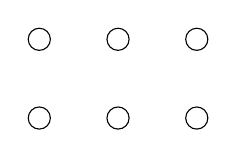
\begin{tikzpicture}
        \draw (0,0) circle (4pt);
        \draw (1,0) circle (4pt);
        \draw (2,0) circle (4pt);
        \draw (0,1) circle (4pt);
        \draw (1,1) circle (4pt);
        \draw (2,1) circle (4pt);
      \end{tikzpicture}
    \end{image}
  \end{hint}
  \begin{hint}
    $3\times 2=6$
  \end{hint}
  \begin{feedback}
    Did you see that there are multiple hints? You can click on the hint button multiple times to see all the hints.

    The answer is $6$, the answer is also $6.0$, $3*2$, $2*4*3/4$, etc., but don't be cheeky and not actually solve the problems.
  \end{feedback}
\end{example}
 
For this course, you should always have a paper and pencil near at
hand to make notes, doodle pictures, or solve complicated equations. You should ALSO have MATLAB open and ready to go, you'll be using it frequently. 

We \textbf{strongly} recommend that you really \textbf{grapple} with a
problem before getting a hint, or moving on.  The difference between
what you learn by struggling with a problem on your own versus
perusing someone else's solution is astonishing.
 
With that said, even if you get an answer right you should
\textbf{always} try the hints out afterwards.  They might explain the
concept from a new point of view, or challenge you to think in a
different way than you solved the problem.
 
 
We support a few different answer types. Here are some example
problems from the different answer types we support:
 
\begin{example} Type in the formula. Notice Ximera tries to render your formula so you can see if you typed it correctly.
  $\frac{x^2+y^2}{7} = \answer{\frac{x^2+y^2}{7}}$
  \begin{feedback}
    Type $\verb|(x^2+y^2)/7|$
  \end{feedback}
\end{example}
 
\begin{example} Type in this formula too!
  $\frac{\tan(x)}{2xa+b^2} = \answer{\frac{\tan(x)}{2xa+b^2} }$
  \begin{feedback}
    Type $\verb|tan(x)/(2xa+b^2)|$
  \end{feedback}
\end{example}
 
\begin{example} And this one! See the feedback
  $\arcsin(x) = \answer{\arcsin(x)}$
  \begin{feedback}
    Type $\verb|arcsin(x)|$
 
    Note that typing $\verb|sin^(-1)(x)|$ does not work.
  \end{feedback}
\end{example}
 
\begin{example} Try this one!
  $|x| = \answer{|x|}$
  \begin{feedback}
    You can type $\verb! |x| !$ or $\verb! abs(x)!$, but
    $\verb! abs(x) !$ may be preferable because it is easier to parse
    appropriately.
  \end{feedback}
\end{example}
\begin{example}
  $\ln(x+1)= \answer{\ln(x+1)}$
  \begin{feedback}
    You could type $\verb|ln(x+1)|$ or $\verb|log(x+1)|$
  \end{feedback}
\end{example}
 
\begin{example} And this!
  $ \sin(\theta) = \answer{\sin(\theta)}$
  \begin{feedback}
    Type $\verb|sin(theta)|$
  \end{feedback}
\end{example}
 
 
\begin{example} Here too!
  $ \varphi = \answer{\varphi}$
  \begin{feedback}
    Type $\verb|phi|$
  \end{feedback}
\end{example}
 
 
\begin{example} Over here!
  $ \rho = \answer{\rho}$
  \begin{feedback}
    Type $\verb|rho|$
  \end{feedback}
\end{example}
 
\begin{example} Hey there sqrt!
    $\sqrt{x} = \answer{\sqrt{x}}$
  \begin{feedback}
    Type $\verb|sqrt(x)|$
  \end{feedback}
  \begin{feedback}
    It would also work to type $\verb| x^(1/2)|$
  \end{feedback}
\end{example}
 
\begin{example} No nth roots here, only fractional powers.
  $\sqrt[3]{y} = \answer{y^{\frac{1}{3}}}$
  \begin{feedback}
    We do not have a ``slick" way to enter this, so you should just
    type $\verb!y^(1/3)!$, which is equivalent.
  \end{feedback}
\end{example}
 
 
\begin{example} Type in the string (aka the word) ``DNE''.
  $DNE = \answer[format=string]{DNE}$
  \begin{feedback}
    Type $\verb|DNE|$.
  \end{feedback}
\end{example}
 
\begin{example}
  $\infty = \answer{\infty}$
  \begin{feedback}
    Type $\verb|infty|$ or $\verb|infinity|$ or $\verb|oo|$.
  \end{feedback}
\end{example}
 
As you complete activities the green ``completion bar'' moves at the
top of the page.  This lets you know how close you are to being done
with an activity.

%include "progress bar"
\begin{center}
  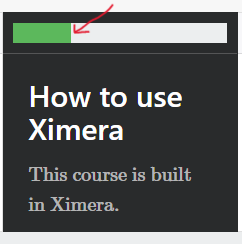
\includegraphics{progress_bar.png}
\end{center}
 
You advance through pages either by completing them and clicking the
``next activity'' button, or by navigating on the little scroll bar at
the top of the page.

We want you to learn from this text. Hence, we ask questions to
``push'' your thinking, and leave blanks in examples to ensure you are
following along. We encourage you to \textbf{keep a notebook} where
you write each question and your answers, along with each major
theorem and example. In essence we want you to imagine that \textbf{we
  are writing mathematics together}, and thus are exploring a new
world of mathematics together.
 
With this in mind, your work is graded on the basis of its correct
\textbf{completion}. The green bar above
\begin{image}
  
\includegraphics{partialBar.png}
\end{image} 
tells you how close you are to completion. We hope that you can
complete each activity and see a full green bar:
\begin{image}
  
\includegraphics{fullGreen.png}
\end{image}
However, sometimes there is a bug that prohibits a ``full green bar.''
In that case, do not despair, as we take these bugs into account when
grading. Moreover, please \textbf{let us know} any issues you are
having. If possible \textbf{we will fix the issue}.
 
If a correction is made then we may make an update. In this case an orange button will appear at the top of the screen:
\begin{image}
  
\includegraphics{update.png}
\end{image}
If you click the ``update'' button, a dialog will appear:
\begin{image}
  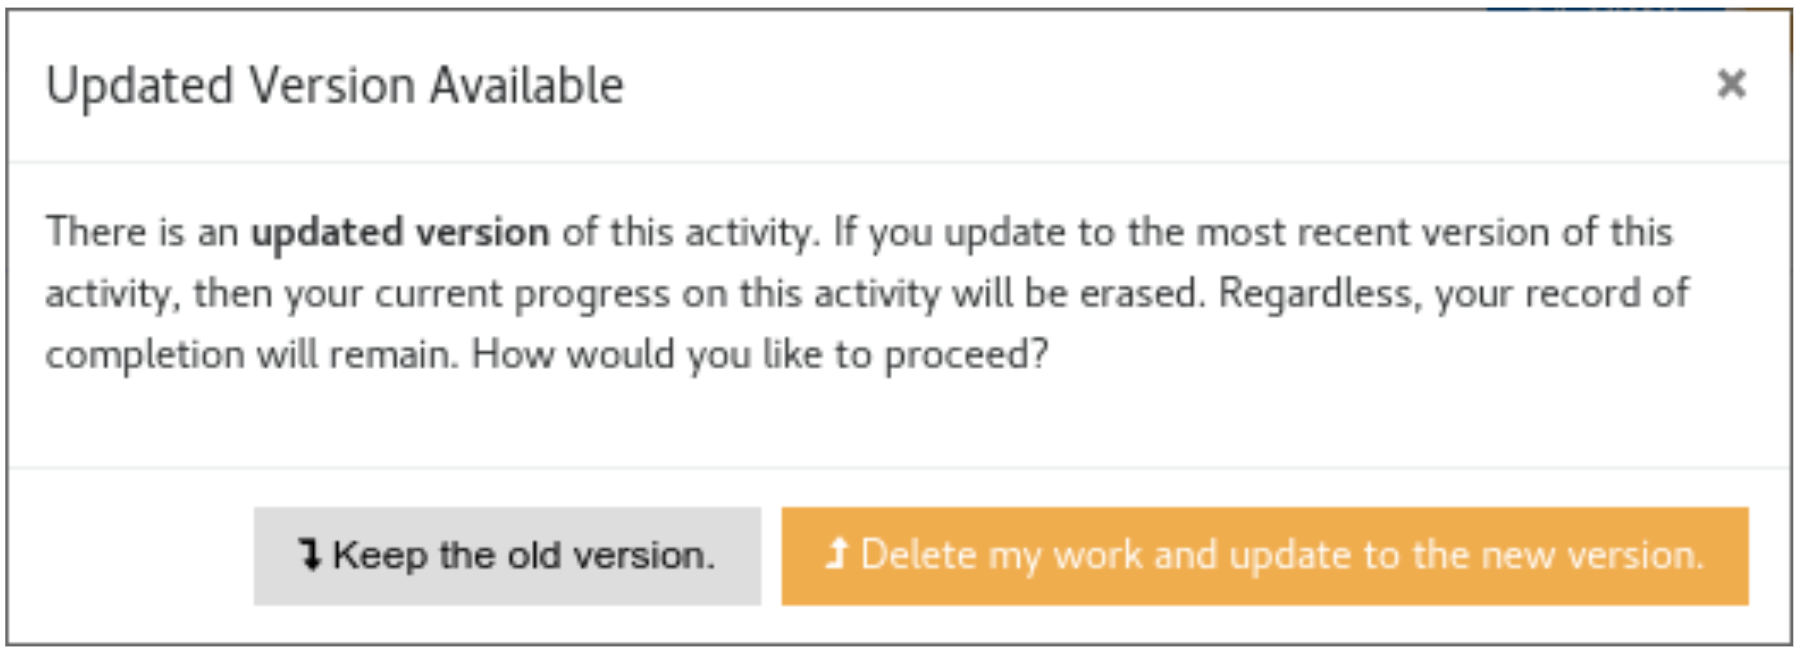
\includegraphics{updateDialog.png}
\end{image}
If you update your work, the current activity will be replaced by a
new activity. Since your previous work was for the previous
incarnation of the activity, your previous work will be
deleted. However, if you've completed the activity, \textbf{your
  record of completion remains}. You can witness this by selecting
another activity, and observing your green-bar for the updated
activity.  Unfortunately, if your activity was not complete before you
updated and you want a full green-bar on the updated activity, you
will have to complete the activity again.
 
 
We simply want you to learn and to provide you with the best possible
learning experience.
 
\subsection*{GeoGebra Interactives}
GeoGebra interactives are one of the most exciting features of this text. You can dynamically visualize and interact with the geometry behind linear algebra, and can even manipulate the objects in the applets to see how the geometry changes. 

Check this out!

\begin{center}
  \geogebra{fxktu8e2}{858}{473}
\end{center}

You can select check boxes and drag points to change a vector's location.

\begin{center}
  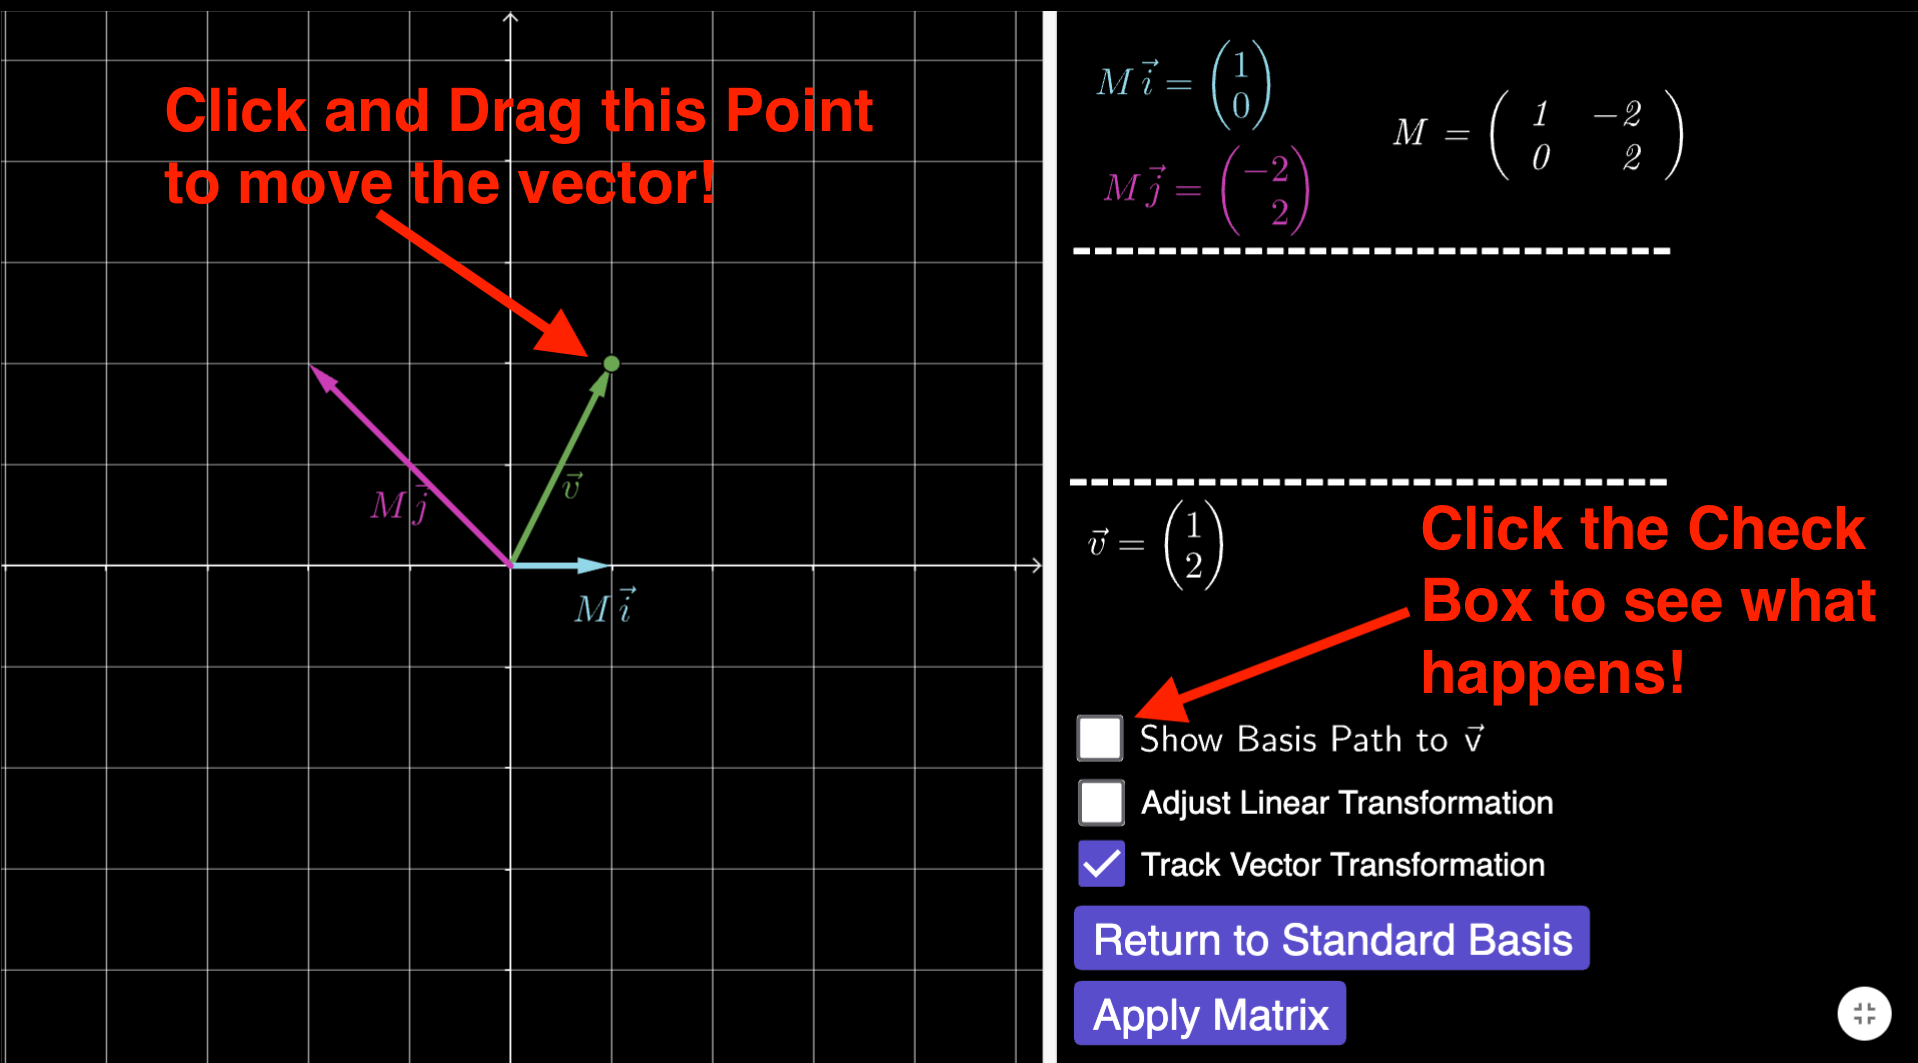
\includegraphics[scale=.25]{gbbEx1.png}
\end{center}

Selecting the check box adds new elements to the screen!

\begin{center}
  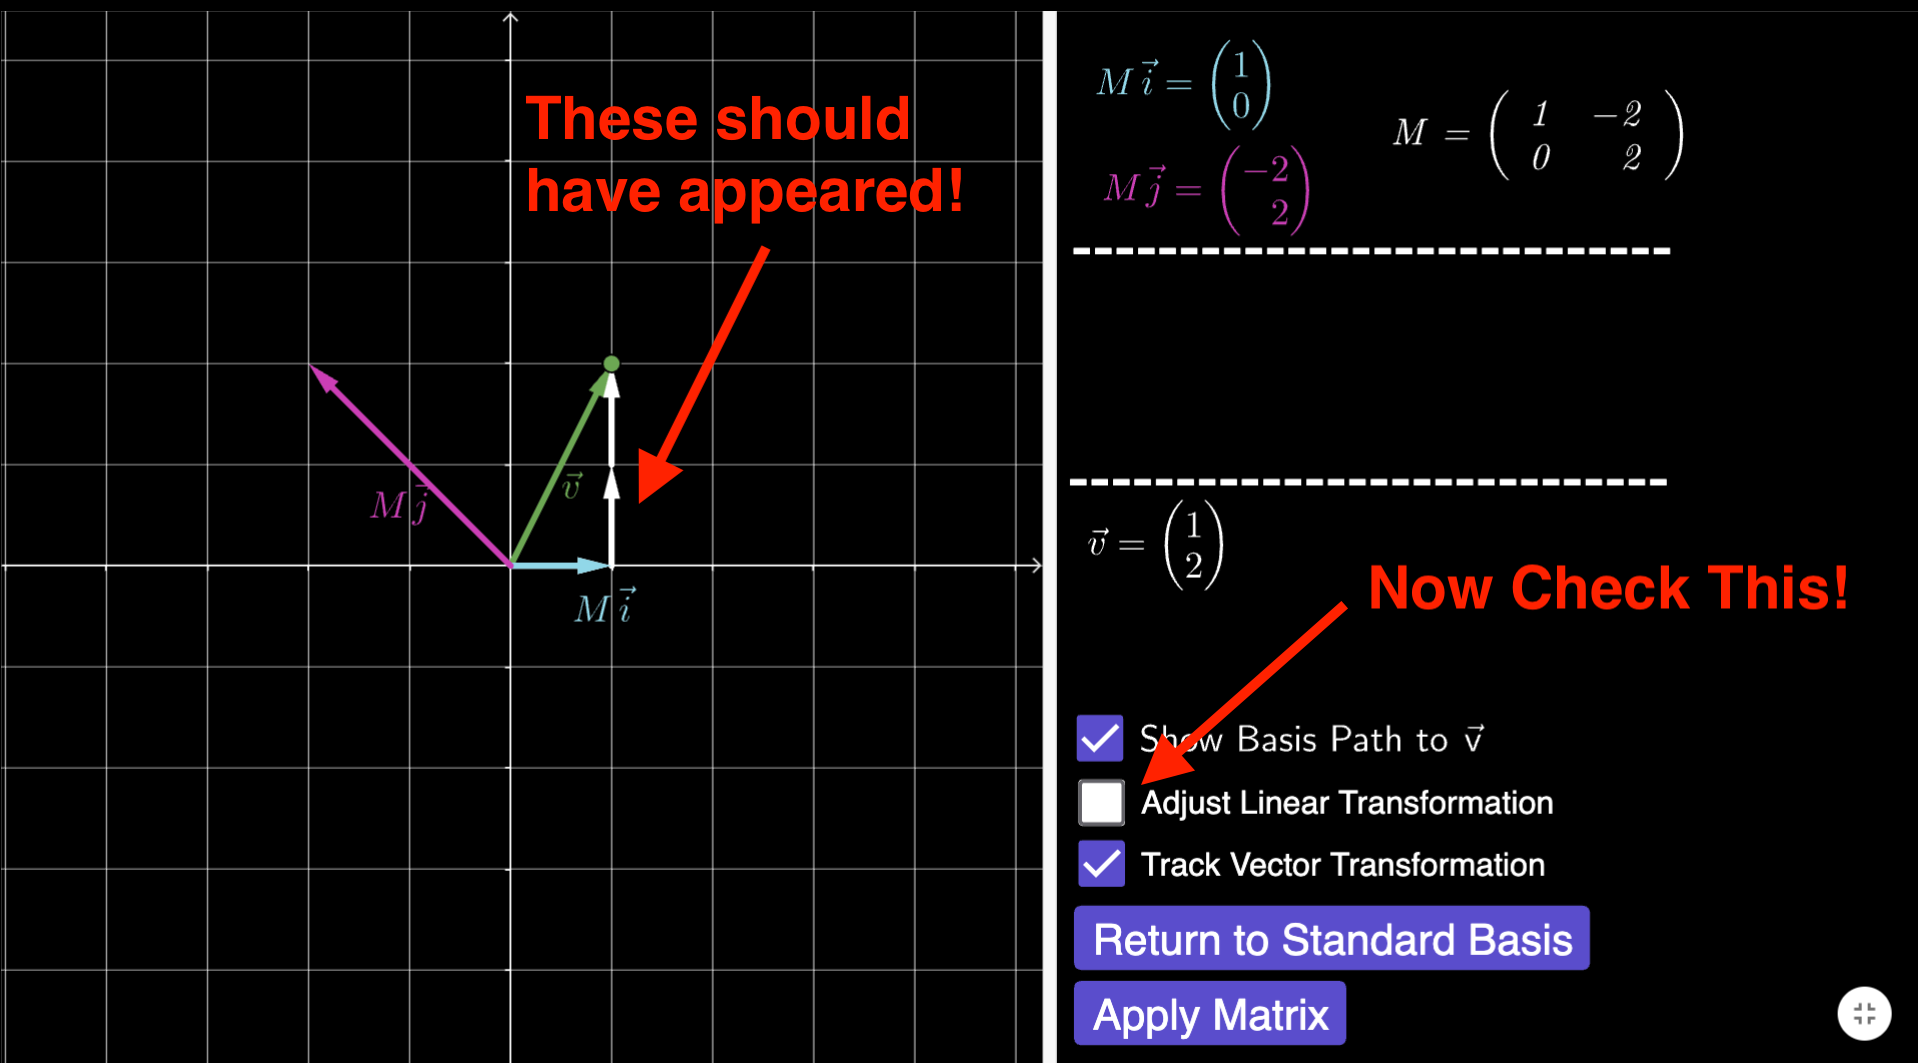
\includegraphics[scale=.25]{gbbEx2.png}
\end{center}

Sometimes check boxes will uncheck other boxes and make new text or interactive elements appear.

\begin{center}
  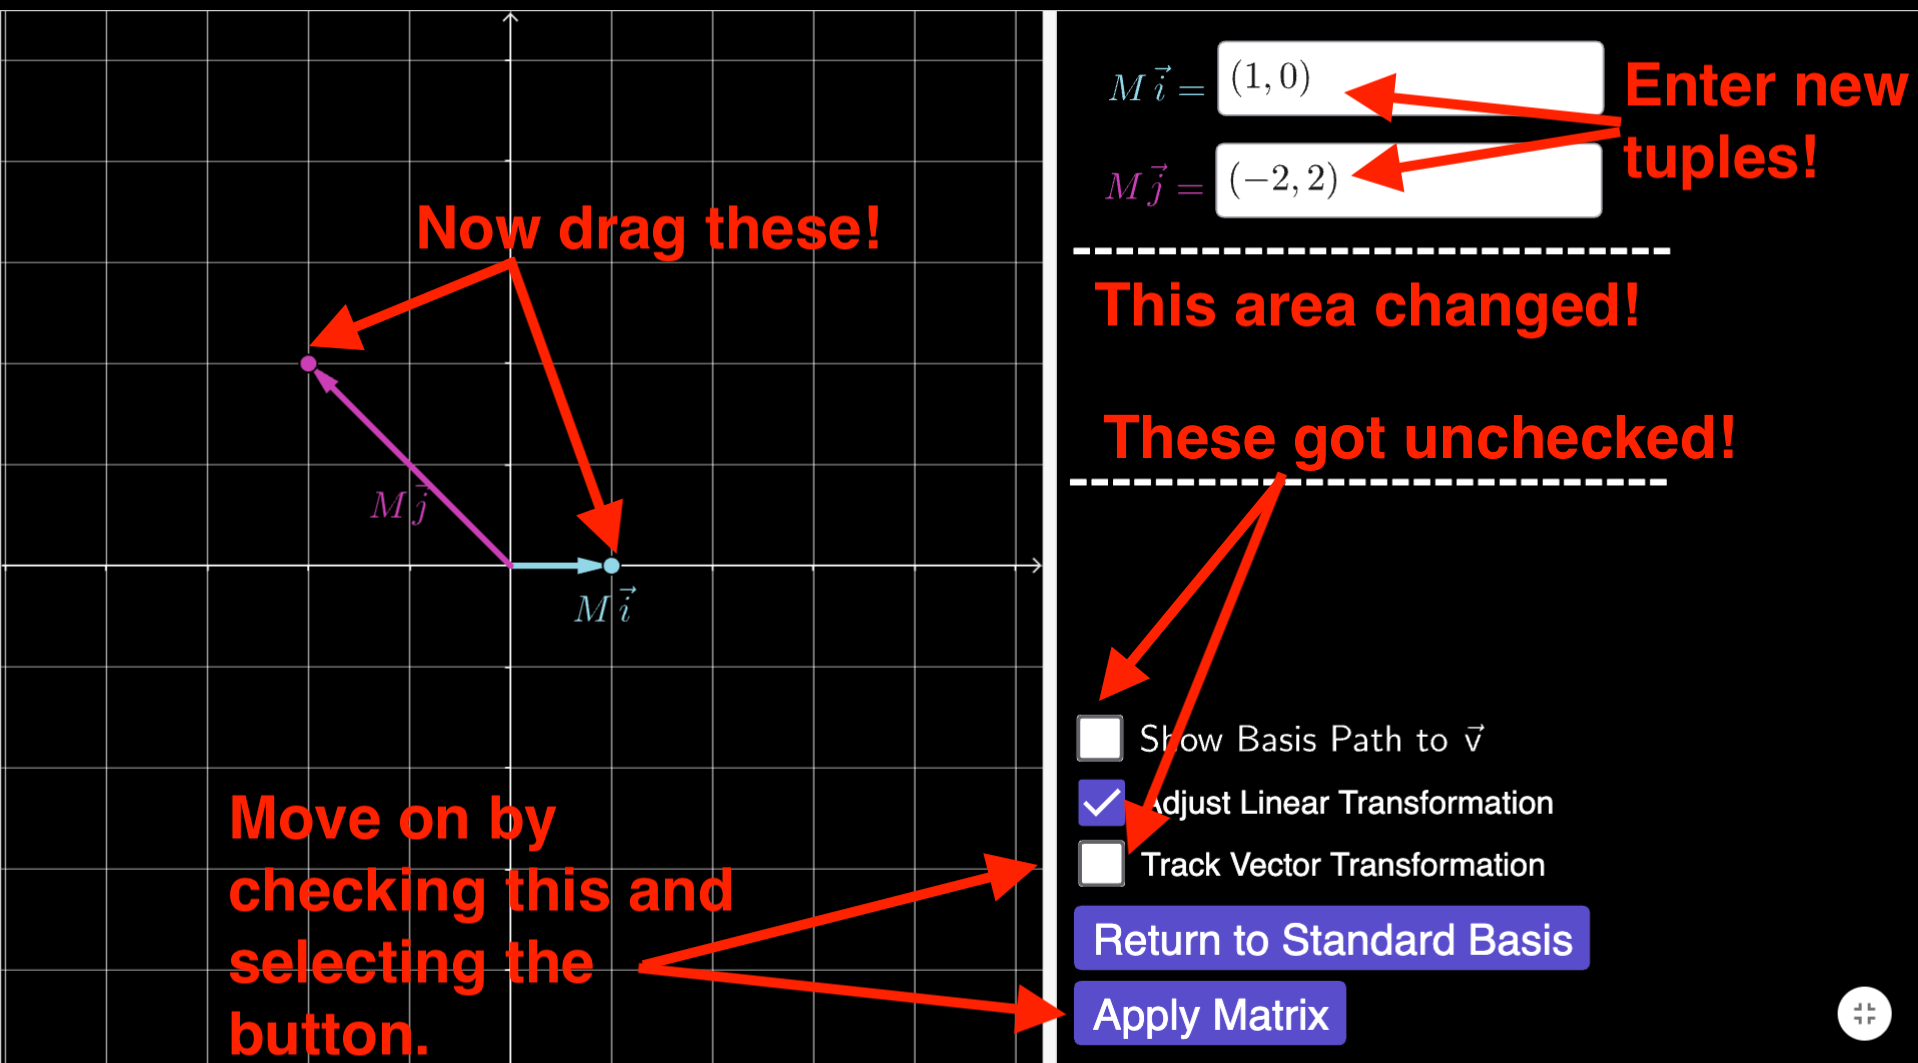
\includegraphics[scale=.25]{gbbEx3.png}
\end{center}

There are also buttons you can push to dynamically alter the screen!

\begin{center}
  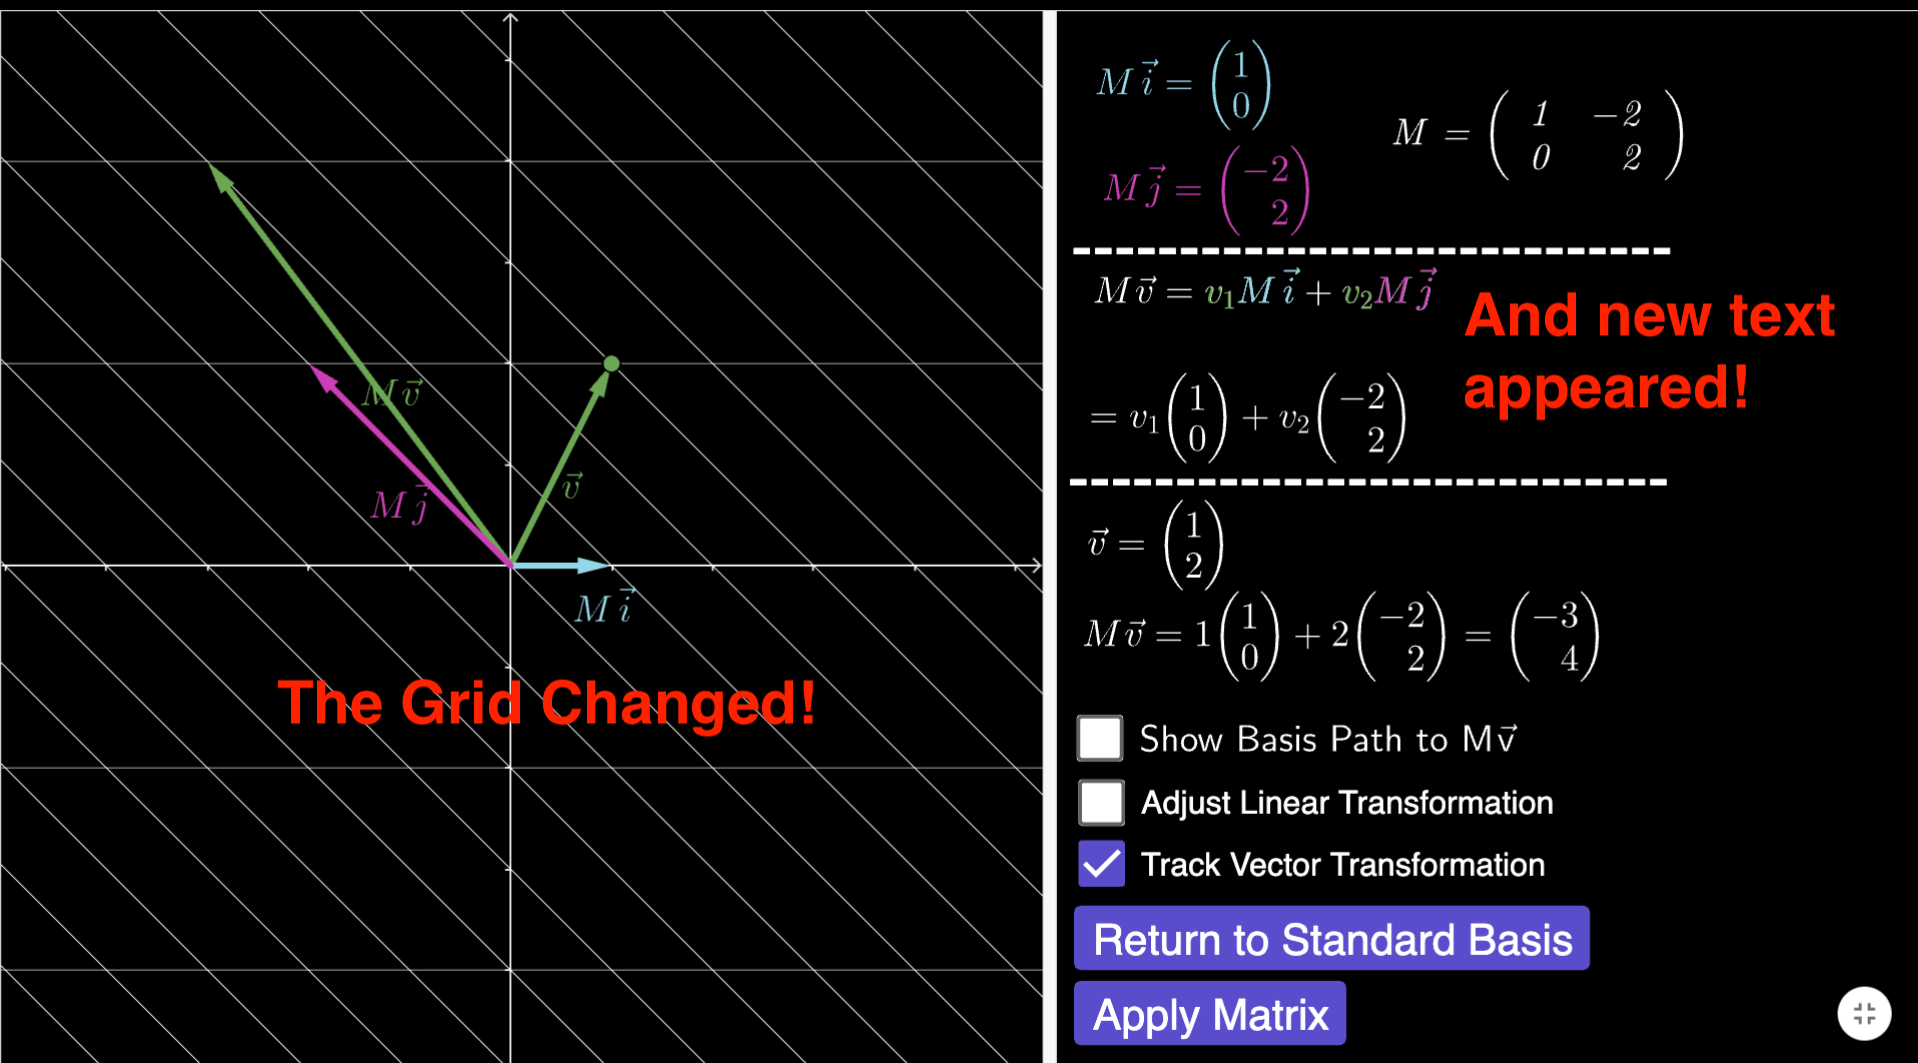
\includegraphics[scale=.25]{gbbEx4.png}
\end{center}

\subsection*{Navigating Ximera}

Most pages will let you navigate to other activities or parts of the text.  

\begin{center}
  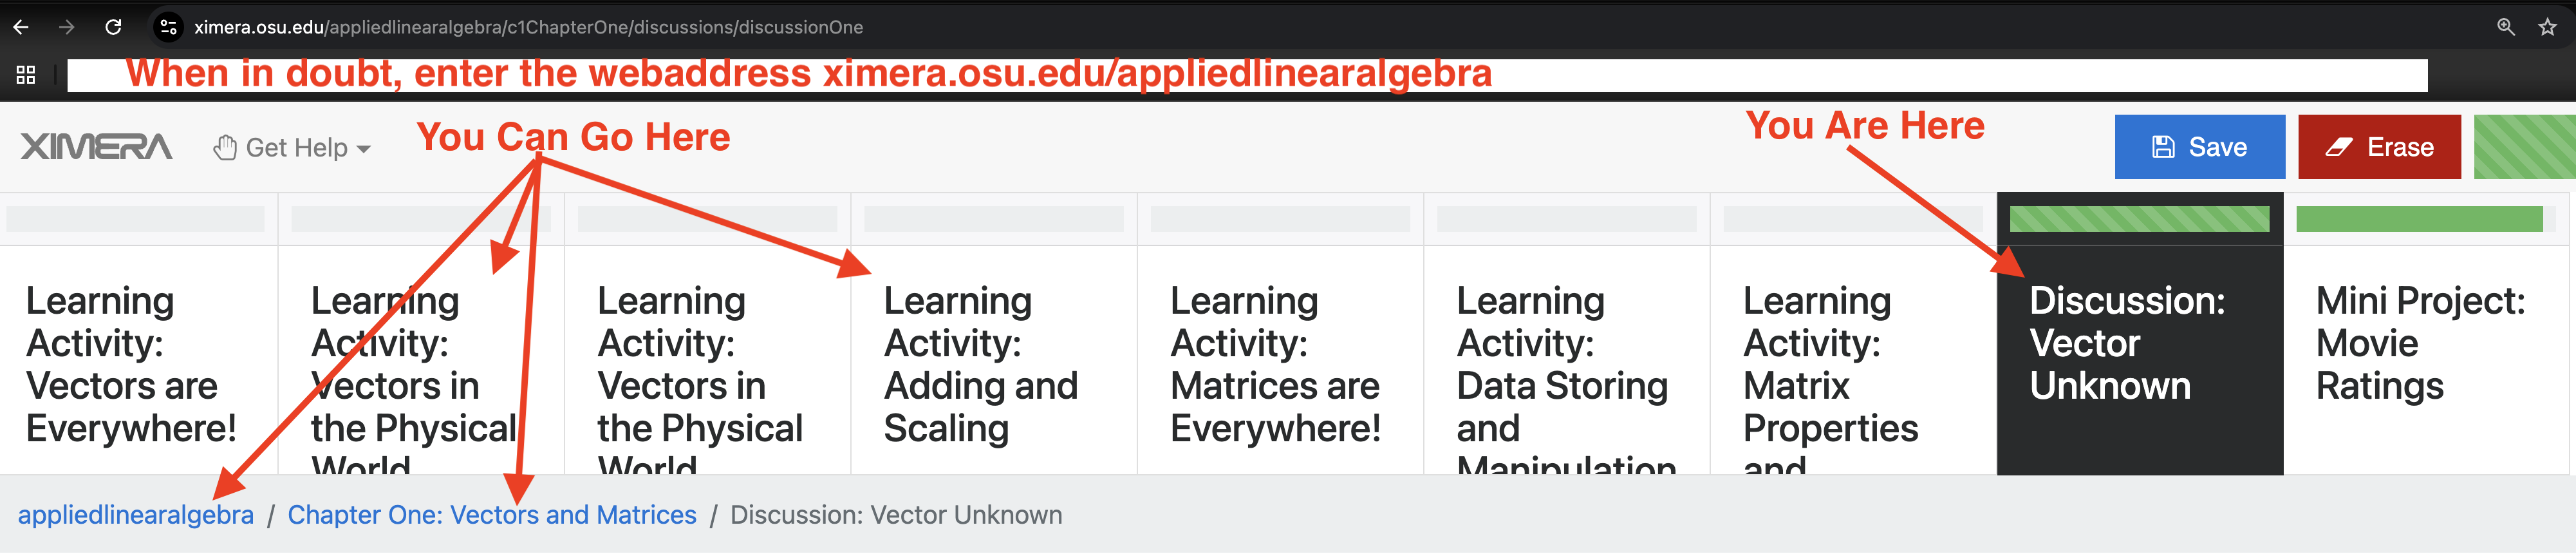
\includegraphics[scale=.25]{navigation1.png}
\end{center}

When in doubt, just type ximera.osu.edu/appliedlinearalgebra in your browser to get to an error screen.

\begin{center}
  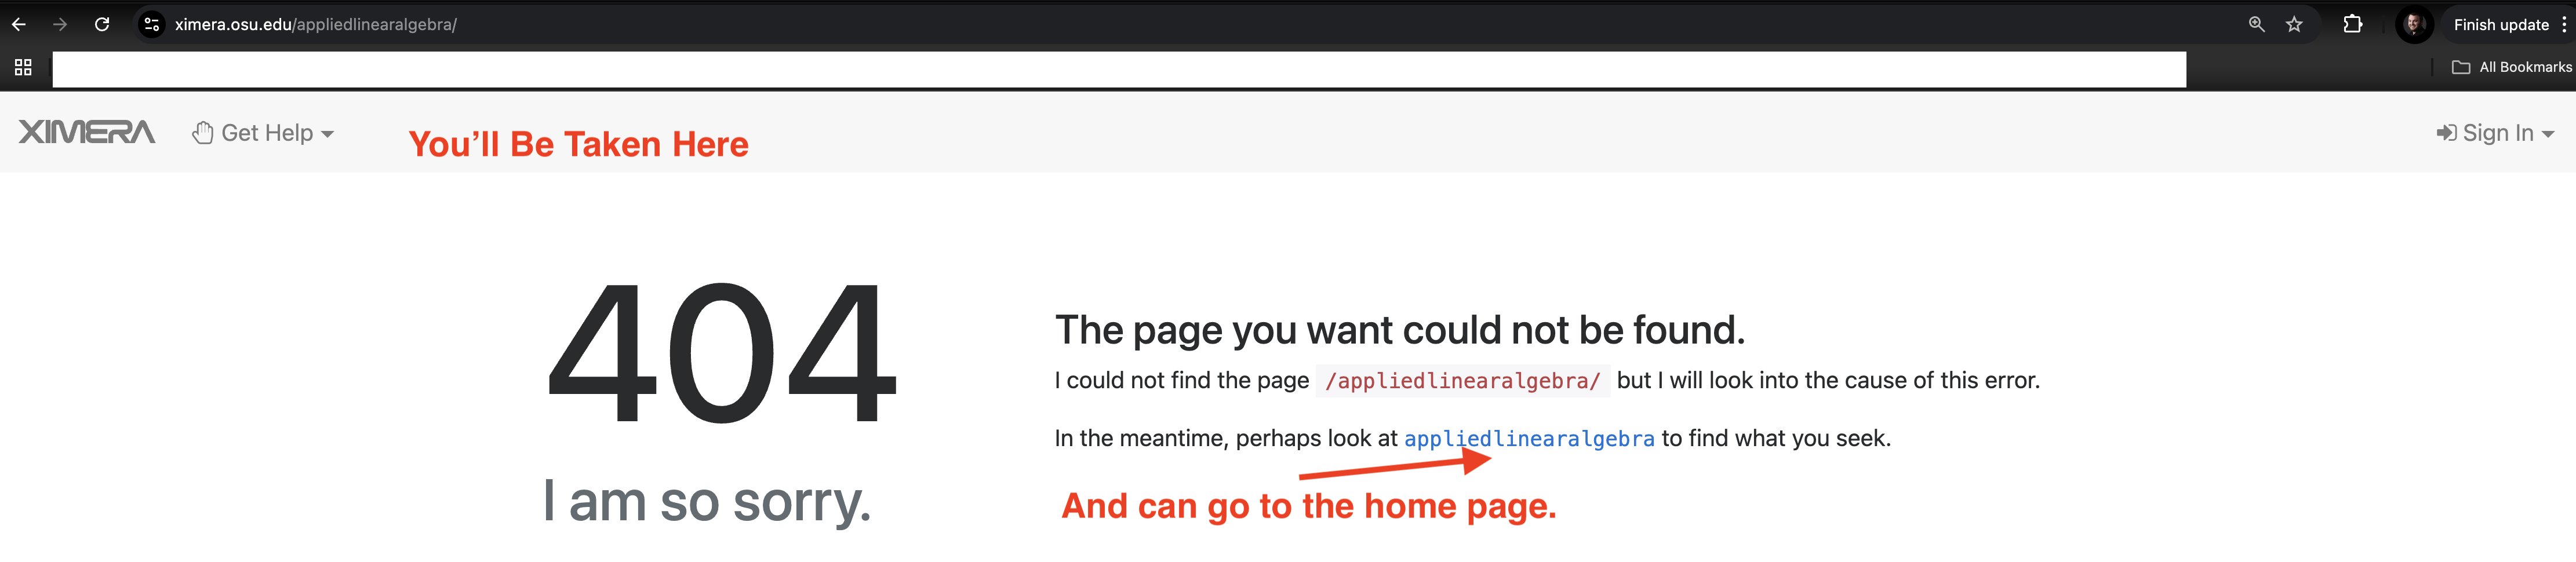
\includegraphics[scale=.25]{navigation2.png}
\end{center}

You can then return to the home page.

\end{document}